\documentclass{beamer}
\usetheme{PaloAlto}
\usepackage{graphicx}
\graphicspath{ {./images/} }

\title[]{Using GitHub Professionally}

\author[]{Liam~Wrubleski\inst{1} \and Marc~Wrubleski\inst{2}}

\institute{
\inst{1}%
BSc. Electrical Engineering, BSc. Mathematics
\and
\inst{2}%
Technical Manager
}

\setbeamercovered{transparent}

\begin{document}
\begin{frame}[plain]
  \maketitle
\end{frame}

\begin{frame}
  \frametitle{Outline}
  \tableofcontents
\end{frame}

\section{What is Github?}
\begin{frame}
  \frametitle{What is Github?}
  What is Git?\pause
  \begin{itemize}[<+->]
    \item Code repository
    \item Version control system
    \item A tool for development
  \end{itemize}
  \vspace{0.25em}
  \uncover<+->{What's the Hub?}
  \begin{itemize}[<+->]
    \item The largest Git server in the world
    \item Showcase of your skills and abilities
    \item History of activity
    \item Collaboration % TODO: what am I saying here?
  \end{itemize}
\end{frame}

\section{Why should I care?}
\begin{frame}
  \frametitle{Why should I care?}
  \framesubtitle{Paradox of Experience}
  Your resume summarizes your experience, your GitHub proves it\\\pause\vspace{0.25em}
  Industry wants experience, but won't hire inexperienced people\\\pause\vspace{0.25em}
  To resolve this, you need your own experience\\\pause\vspace{0.25em}
  Work on problems, already solved or not, and record the process!
\end{frame}

\section{How do I use GitHub?} % GitHub Desktop

\begin{frame}
	\frametitle{How do I use GitHub?}
	\framesubtitle{Setting Expectations}
	\begin{figure}
		\label{https://xkcd.com/1597/}
		\centering
		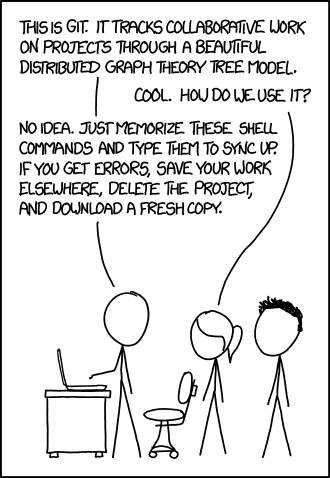
\includegraphics[height=0.8\textheight]{xkcd-git}
	\end{figure}
\begin{flushright}
	\footnotesize{https://xkcd.com/1597}
\end{flushright}
\end{frame}

\begin{frame}
  \frametitle{How do I use GitHub?}
  \framesubtitle{The Basics}
  On GitHub, your work is organized into repositories, or "repos".\\\pause\vspace{0.25em}
  When you start a new project, you start a new repo.\\\pause\vspace{0.25em}
  % Here we show starting a new repo
  Many ways to work with repos:
  \begin{itemize}[<+->]
    \item In-browser
    \item GitHub Desktop
    \item Command line
  \end{itemize}
\end{frame}

\begin{frame}
  \frametitle{How do I use GitHub?}
  \framesubtitle{Branches}
  GitHub lets you create "branches" on your project\\\pause\vspace{0.25em}
  To begin with, you work with the "master" branch\\\pause\vspace{0.25em}
  Branches start out identical to what they branched from\\\pause\vspace{0.25em}

  \begin{alertblock}{Push to master?}
    Working on the master branch is generally strongly discouraged. Think of pushing to the master branch as releasing a new version, you don't want to do it until you're sure it's ready.
  \end{alertblock}
\end{frame}

\begin{frame}
  \frametitle{How do I use GitHub?}
  \framesubtitle{Merging}
  You can work as long as you want on any particular branch\\\pause\vspace{0.25em}
  When you want to move your changes to another branch, you "merge"\\\pause\vspace{0.25em}
  This is sometimes simple, and sometimes complex\\\vspace{0.25em}
\end{frame}

\begin{frame}
  \frametitle{How do I use GitHub?}
  \framesubtitle{Forking and pull requests}
  GitHub loves open source, so anyone can contribute to pretty much anything!\\\pause\vspace{0.25em}
  If you want to contribute to a project, here's the workflow:
  \begin{enumerate}[<+->]
    \item Fork
    \item Branch
    \item Work
    \item Pull request
  \end{enumerate}\pause
  Pull requests are just you asking the developer to merge your changes
\end{frame}

\section{How do I make a good profile?}
\begin{frame}
  \frametitle{How do I make a good profile?}
  \framesubtitle{Contribution History}
  Your GitHub account tracks your contribution history\\\pause\vspace{0.25em}
  Having a long and consistent contribution history is valuable\\\pause\vspace{0.25em}
  One very good thing you can do for your profile is to consistently work on things!
\end{frame}

\begin{frame}
  \frametitle{How do I make a good profile?}
  \framesubtitle{Information}
  \textbf{What should you set?}\pause
  \begin{itemize}[<+->]
    \item Name
    \item Contact information
    \item Biography
    \begin{itemize}
      \item Short (160 characters)
      \item Grab the reader's attention
      \item Highlight your skills, education, or passions
    \end{itemize}
  \end{itemize}
\end{frame}

\begin{frame}
  \frametitle{How do I make a good profile?}
  \framesubtitle{Repositories}
  Your repositories all should have a README.md\\\vspace{0.25em}
  Having nice READMEs demonstrates that you can keep good documentation.\\\pause\vspace{0.25em}
  You can have up to 6 of your public repositories pinned on your profile.\pause\\
  \textbf{What should you pin?}
  \begin{itemize}[<+->]
    \item Projects emphasizing your skills
    \item Projects you're proud of
    \item Popular repositories
  \end{itemize}
\end{frame}

\begin{frame}
  \frametitle{How do I make a good profile?}
  \framesubtitle{What not to include}
  Don't include more non-professional information than necessary\\\pause\vspace{0.25em}
  This accomplishes two things:
  \begin{itemize}[<+->]
    \item Keeps professional tools professional
    \item Minimizes the influence of any unconscious bias your reader might have
  \end{itemize}
\end{frame}

\begin{frame}
  \frametitle{How do I make a good profile?}
  \framesubtitle{README.md}
  GitHub has a secret feature on a repo with your username\\\vspace{0.25em}
  The README will be on your profile, giving you some more flexibility\\\vspace{0.25em}
  Uses Markdown, the same as any other repository\\\pause\vspace{0.25em}
  To use this, create a repo with the same name as your username, and set README.md there
  % TODO: reduce wordiness
\end{frame}

\section{Work with it!} % TODO: rename
\begin{frame}
  \frametitle{Questions?}
  Thanks for your attention!
\end{frame}
\end{document}
